\let\negmedspace\undefined
\let\negthickspace\undefined
\documentclass[journal,12pt,onecolumn]{IEEEtran}
\usepackage{cite}
\usepackage{amsmath,amssymb,amsfonts,amsthm}
\usepackage{algorithmic}
\usepackage{graphicx}
\graphicspath{{./figs/}}
\usepackage{textcomp}
\usepackage{xcolor}
\usepackage{txfonts}
\usepackage{listings}
\usepackage{enumitem}
\usepackage{mathtools}
\usepackage{gensymb}
\usepackage{comment}
\usepackage{caption}
\usepackage[breaklinks=true]{hyperref}
\usepackage{tkz-euclide} 
\usepackage{listings}
\usepackage{gvv}                                        
%\def\inputGnumericTable{}                                 
\usepackage[latin1]{inputenc}     
\usepackage{xparse}
\usepackage{color}                                            
\usepackage{array}
\usepackage{longtable}                                       
\usepackage{calc}                                             
\usepackage{multirow}
\usepackage{multicol}
\usepackage{hhline}                                           
\usepackage{ifthen}                                           
\usepackage{lscape}
\usepackage{tabularx}
\usepackage{array}
\usepackage{float}
\newtheorem{theorem}{Theorem}[section]
\newtheorem{problem}{Problem}
\newtheorem{proposition}{Proposition}[section]
\newtheorem{lemma}{Lemma}[section]
\newtheorem{corollary}[theorem]{Corollary}
\newtheorem{example}{Example}[section]
\newtheorem{definition}[problem]{Definition}
\newcommand{\BEQA}{\begin{eqnarray}}
\newcommand{\EEQA}{\end{eqnarray}}
\newcommand{\define}{\stackrel{\triangle}{=}}
\theoremstyle{remark}
\newtheorem{rem}{Remark}

\begin{document}
\title{1.5.32}
\author{EE25BTECH11045 - P.Navya Priya}
\maketitle
\renewcommand{\thefigure}{\theenumi}
\renewcommand{\thetable}{\theenumi}

\vspace{1cm}

 Find the ratio in which the line segment joining the points $(1,-3)$ and $(4,5)$ is divided
 by X axis.

\vspace{0.75cm}
\textbf{Solution:} Let $\vec{A}$ = \myvec{1\\-3} and $\vec{C}$ = \myvec{4\\5}\\[5pt]

Consider a point $\vec{B}$ = \myvec{$x$\\0} on the X-axis.
As the points $\vec{A,B,C}$ are collinear
The matrix 

$\myvec{ \vec{B}-\vec{A} & \vec{C}-\vec{A} }^\top$ has rank 1.
\begin{align}
\myvec{ \vec{B}-\vec{A} & \vec{C}-\vec{A} }^\top = \myvec{3&x-1\\8&3}^\top
\end{align}
\begin{align}
\myvec{ \vec{B}-\vec{A} & \vec{C}-\vec{A} }^\top = \myvec{3&8\\x-1&3}
\end{align}
\begin{align}
\myvec{3&8\\x-1&3}
 &\xleftrightarrow{R_2 = 8R_2 - 3R_1}
 \myvec{3&8\\8(x-1)-9&0}
\end{align}
\begin{align}
\xleftrightarrow{R_{1}\rightarrow\frac{R_{1}}{3}}\myvec{1&\frac{8}{3}\\8x-17&0}
\end{align}
\begin{align}
\xleftrightarrow{R_{2}\rightarrow R_{2}-\brak{8x-17}R_{1}}\myvec{1&\frac{8}{3}\\[3pt]0&\frac{8\brak{17-8x}}{3}}
\end{align}

 To satisfy collinearity condition, the rank of above matrix should be 1. Hence,
\begin{align}
\frac{8\brak{17-8x}}{3} = 0
\end{align}

\begin{align}
    x = 17/8
\end{align}


Assume the ratio $\vec{B}$ divides $\vec{A}$  and $\vec{C}$ be k:1

\begin{align}
    k = \frac{\myvec{\vec{A} - \vec{B}}^\top \myvec{\vec{B} - \vec{C}}}{||\myvec{\vec{B} - \vec{C}}||^2}
\end{align}

Substituting the values of $\vec{A}, \vec{B} \, and \, \vec{C}$

\begin{align}
    k = \frac{1095}{1825}
\end{align}

\begin{align}
    k = \frac{3}{5}
\end{align}

\centering
\begin{large}Hence the ratio is 3:5.\end{large}

\vspace{0.5cm}
\begin{figure}[H]
\centering
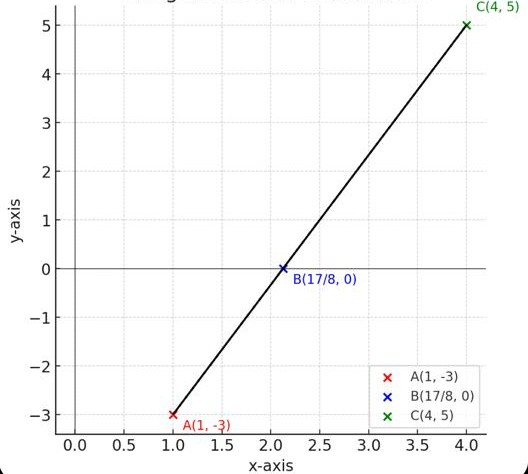
\includegraphics[width=0.8\columnwidth]{figs/graph.png}
 \caption*{Plot of Intersection of AB by X-axis}
\label{fig:graph.png}
\end{figure}
\end{document}
















